\section{\KLUDGE 概要}

\index{Collision}
Collision\KLUDGE モジュールは物理計算の基礎となる衝突判定機能を提供します.
\KLUDGE 事実上Collision\KLUDGE モジュールはPhysics\KLUDGE モジュールのサブモジュールとなっており,両者は密接に依存しています.
\KLUDGE ユーザは主として剛体に衝突判定用形状を割り当てる際にCollision\KLUDGE モジュールの機能を利用することになります.

\begin{figure}[t]
\begin{center}
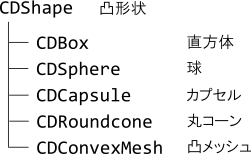
\includegraphics[width=.4\hsize]{fig/cdclass.eps}
\end{center}
\caption{Class hierarchy of Collision module}
\label{fig_cdclass}
\end{figure}

\index{CDShape}
Collision\KLUDGE モジュールのクラス階層をFig.\,\ref{fig_cdclass}\KLUDGE に示します.
\KLUDGE 衝突判定形状はすべて\url{CDShape}\KLUDGE から派生します.
\KLUDGE アルゴリズムの性質上,形状はすべて凸形状でなければなりません.

\section{\KLUDGE 形状の作成}

\KLUDGE 衝突判定形状は次の手順で作成・登録します.
\begin{enumerate}
\item \KLUDGE 形状を作成する
\item \KLUDGE 剛体へ形状を追加する
\item \KLUDGE 形状の位置を設定する
\end{enumerate}
\KLUDGE 以下に順を追って説明します.

\KLUDGE まず形状を作成するには次のようにします.
\begin{sourcecode}
// given PHSdkIf* phSdk

CDBoxDesc desc;
desc.boxsize = Vec3d(1.0, 1.0, 1.0);

CDBoxIf* box = phSdk->CreateShape(desc)->Cast();
\end{sourcecode}
\KLUDGE 衝突判定形状のオブジェクトはPhysics\KLUDGE モジュールが管理します.
\KLUDGE このため,形状を作成するには\url{PHSdk}\KLUDGE クラスの\url{CreateShape}\KLUDGE 関数を使います.
\url{PHSdk}\KLUDGE については\ref{chap_physics}\KLUDGE 章を参照してください.
\KLUDGE 形状を作成するには,まず種類に応じたディスクリプタを作成し,寸法などのパラメータを設定します.
\KLUDGE この例では直方体クラス\url{CDBox}\KLUDGE のディスクリプタを作成して一辺が$1.0$\KLUDGE の立方体を作成します.
\KLUDGE ディスクリプタを指定して\url{CreateShape}\KLUDGE を呼び出すと,対応する種類の形状が作成され,
\KLUDGE そのインタフェースが返されます.
\KLUDGE ただし戻り値は形状の基底クラスである\url{CDShape}\KLUDGE のインタフェースですので,派生クラス(ここでは\url{CDBox}\KLUDGE )のインタフェースを得るには
\KLUDGE 上のように\url{Cast}\KLUDGE 関数で動的キャストする必要があります.

\KLUDGE 形状を作成したら,次にその形状を与えたい剛体に登録します.
\begin{sourcecode}
// given PHSolidIf* solid

solid->AddShape(box);         // first box
\end{sourcecode}
\KLUDGE 剛体クラス\url{PHSolid}\KLUDGE については\ref{chap_physics}\KLUDGE 章を参照してください.
\KLUDGE ここで重要なことは,一度作成した形状は1\KLUDGE つの剛体にいくつでも登録でき,また異なる複数の剛体にも登録できるということです.
\KLUDGE つまり,同じ形状を複数の剛体間で共有することで,形状の作成コストやメモリ消費を抑えることができます.

\url{AddShape}\KLUDGE 関数で登録した直後の形状は,剛体のローカル座標系の原点に位置しています.
\KLUDGE これを変更したい場合は\url{SetShapePose}\KLUDGE 関数を使います.
\begin{sourcecode}
solid->AddShape(box);         // second box
solid->AddShape(box);         // third box 

// move first shape 1.0 in x-direction
solid->SetShapePose(0, Posed(Vec3d(1.0, 0.0, 0.0), Quaterniond());

// rotate second shape 30 degrees along y-axis
solid->SetShapePose(1, Posed(Vec3d(),
                    Quaterniond::Rot(Rad(30.0), 'y')));
\end{sourcecode}
\url{SetShapePose}\KLUDGE の第1\KLUDGE 引数は操作する形状の番号です.最初に\url{AddShape}\KLUDGE した形状の番号が$0$\KLUDGE で,\url{AddShape}\KLUDGE するたびに$1$\KLUDGE 増加します.
\KLUDGE 形状の位置や向きは剛体のローカル座標系で指定します.
\KLUDGE また,形状の位置・向きを取得するには\url{GetShapePose}\KLUDGE 関数を使います.

\KLUDGE 以下ではSpringhead\KLUDGE でサポートされている形状を種類別に解説します.

\subsection*{\KLUDGE 直方体}

\begin{figure}[t]
\begin{center}
\includegraphics[width=.4\hsize]{fig/cdbox.eps}
\end{center}
\caption{Box geometry}
\label{fig_cdbox}
\end{figure}

\index{CDBox}
\index{\KLUDGE ちょくほうたい@\KLUDGE 直方体}
\KLUDGE 直方体(Fig.\,\ref{fig_cdbox})\KLUDGE のクラスは\texttt{CDBox}\KLUDGE です.

\begin{center}
\begin{tabular}{lll}
\multicolumn{3}{l}{\texttt{CDBoxDesc}}					\\ \midrule
\texttt{Vec3f}	&	\texttt{boxsize}	& \KLUDGE 各辺の長さ 	\\
\\
\multicolumn{3}{l}{\texttt{CDBoxIf}}					\\ \midrule
\multicolumn{2}{l}{\texttt{Vec3f GetBoxSize()}}			\\
\multicolumn{2}{l}{\texttt{void SetBoxSize(Vec3f)}}		\\
\end{tabular}
\end{center}


\subsection*{\KLUDGE 球}

\begin{figure}[t]
\begin{center}
\includegraphics[width=.4\hsize]{fig/cdsphere.eps}
\end{center}
\caption{Sphere geometry}
\label{fig_cdsphere}
\end{figure}

\index{CDSphere}
\index{\KLUDGE きゅう@\KLUDGE 球}
\KLUDGE 球(Fig.\,\ref{fig_cdsphere})\KLUDGE のクラスは\url{CDSphere}\KLUDGE です.

\begin{center}
\begin{tabular}{lll}
\multicolumn{3}{l}{\texttt{CDSphereDesc}}				\\ \midrule
\texttt{float}	&	\texttt{radius}	& \KLUDGE 半径 				\\
\\
\multicolumn{3}{l}{\texttt{CDSphereIf}}					\\ \midrule
\multicolumn{2}{l}{\texttt{float GetRadius()}}			\\
\multicolumn{2}{l}{\texttt{void SetRadius(float)}}		\\
\end{tabular}
\end{center}


\subsection*{\KLUDGE カプセル}

\begin{figure}[t]
\begin{center}
\includegraphics[width=.4\hsize]{fig/cdcapsule.eps}
\end{center}
\caption{Capsule geometry}
\label{fig_cdcapsule}
\end{figure}

\index{CDCapsule}
\index{\KLUDGE かぷせる@\KLUDGE カプセル}
\KLUDGE カプセル(Fig.\,\ref{fig_cdcapsule})\KLUDGE のクラスは\url{CDCapsule}\KLUDGE です.
\KLUDGE カプセルは円柱の両端に半球がついた形をしています.

\begin{center}
\begin{tabular}{lll}
\multicolumn{3}{l}{\texttt{CDCapsuleDesc}}				\\ \midrule
\texttt{float}	&	\texttt{radius}	& \KLUDGE 半球の半径 		\\
\texttt{float}	&	\texttt{length} & \KLUDGE 円柱の長さ		\\
\\
\multicolumn{3}{l}{\texttt{CDCapsuleIf}}				\\ \midrule
\multicolumn{2}{l}{\texttt{float GetRadius()}}			\\
\multicolumn{2}{l}{\texttt{void SetRadius(float)}}		\\
\multicolumn{2}{l}{\texttt{float GetLength()}}			\\
\multicolumn{2}{l}{\texttt{void SetLength(float)}}		\\
\end{tabular}
\end{center}


\subsection*{\KLUDGE 丸コーン}

\begin{figure}[t]
\begin{center}
\includegraphics[width=.4\hsize]{fig/cdroundcone.eps}
\end{center}
\caption{Round cone geometry}
\label{fig_cdroundcone}
\end{figure}

\index{CDRoundCone}
\index{\KLUDGE まるこーん@\KLUDGE 丸コーン}
\KLUDGE 丸コーン(Fig.\,\ref{fig_cdroundcone})\KLUDGE のクラスは\url{CDRoundCone}\KLUDGE です.
\KLUDGE 丸コーンはカプセルの両端の半径が非対称になったものです.

\begin{center}
\begin{tabular}{lll}
\multicolumn{3}{l}{\texttt{CDRoundConeDesc}}			\\ \midrule
\texttt{Vec2f}	&	\texttt{radius}	& \KLUDGE 各半球の半径		\\
\texttt{float}	&	\texttt{length} & \KLUDGE 半球間の距離		\\
\\
\multicolumn{3}{l}{\texttt{CDRoundConeIf}}				\\ \midrule
\multicolumn{2}{l}{\texttt{Vec2f GetRadius()}}			\\
\multicolumn{2}{l}{\texttt{void SetRadius(Vec2f)}}		\\
\multicolumn{2}{l}{\texttt{float GetLength()}}			\\
\multicolumn{2}{l}{\texttt{void SetLength(float)}}		\\
\multicolumn{2}{l}{\texttt{void SetWidth(Vec2f)}}		\\
\end{tabular}
\end{center}

\texttt{SetWidth}\KLUDGE 関数は,丸コーンの全長を保存したまま半径を変更します.


\subsection*{\KLUDGE 凸メッシュ}

\begin{figure}[t]
\begin{center}
\includegraphics[width=.4\hsize]{fig/cdconvexmesh.eps}
\end{center}
\caption{Convex mesh geometry}
\label{fig_cdconvexmesh}
\end{figure}

\index{CDConvexMesh}
\index{\KLUDGE とつめっしゅ@\KLUDGE 凸メッシュ}
\KLUDGE 凸メッシュ(Fig.\,\ref{fig_cdconvexmesh})\KLUDGE のクラスは\url{CDConvexMesh}\KLUDGE です.
\KLUDGE 凸メッシュとは凹みや穴を持たない多面体です.
\KLUDGE 頂点座標を指定することで自由な形を作成することができます.

\begin{center}
\begin{tabular}{lll}
\multicolumn{3}{l}{\texttt{CDConvexMeshDesc}}						\\ \midrule
\texttt{vector<Vec3f>}	&	\texttt{vertices}	& \KLUDGE 頂点座標の配列	\\
\\
\multicolumn{3}{l}{\texttt{CDConvexMeshIf}}					\\ \midrule
\multicolumn{2}{l}{\texttt{Vec3f* GetVertices()}}			& \KLUDGE 頂点配列の先頭アドレス	\\
\multicolumn{2}{l}{\texttt{int NVertex()}}					& \KLUDGE 頂点数					\\
\multicolumn{2}{l}{\texttt{CDFaceIf* GetFace(int i)}}		& $i$\KLUDGE 番目の面				\\
\multicolumn{2}{l}{\texttt{int NFace()}}					& \KLUDGE 面数						\\
\end{tabular}
\end{center}

\KLUDGE 凸メッシュが作成される際,\texttt{CDConvexMeshDesc::vertices}\KLUDGE に格納された頂点を内包する最小の凸多面体(凸包)が作成されます.
\KLUDGE 多面体の面を表す\texttt{CDFace}\KLUDGE のインタフェースを以下に示します.

\begin{center}
\begin{tabular}{lll}
\multicolumn{3}{l}{\texttt{CDFaceIf}}						\\ \midrule
\multicolumn{2}{l}{\texttt{int* GetIndices()}}				& \KLUDGE 頂点インデックス配列の先頭アドレス	\\
\multicolumn{2}{l}{\texttt{int NIndex()}}					& \KLUDGE 面の頂点数							\\
\end{tabular}
\end{center}

\texttt{NIndex}\KLUDGE は面を構成する頂点の数を返します(通常$3$\KLUDGE か$4$\KLUDGE です).
\KLUDGE 面は頂点配列を直接保有せず,インデックス配列として間接的に頂点を参照します.
\KLUDGE したがって,面の頂点座標を得るには
\begin{sourcecode}
// given CDConvexMeshIf* mesh
CDFaceIf* face = mesh->GetFace(0);        // get 0-th face
int* idx = face->GetIndices();
Vec3f v = mesh->GetVertices()[idx[0]];    // get 0-th vertex
\end{sourcecode}
\KLUDGE とします.

\section{\KLUDGE 物性の指定}
\label{sec_collision_material}

\index{PHMaterial}
\index{\KLUDGE ぶっせい@\KLUDGE 物性}
\KLUDGE 形状には摩擦係数や跳ね返り係数などの物性を指定することができます.
\KLUDGE 形状の基本クラスである\texttt{CDShape}\KLUDGE のディスクリプタ\texttt{CDShapeDesc}\KLUDGE は\texttt{PHMaterial}\KLUDGE 型の変数\texttt{material}\KLUDGE を持っています.

\begin{center}
\begin{tabular}{lll}
\multicolumn{3}{l}{\texttt{PHMaterial}}							\\ \midrule
\texttt{float}	&	\texttt{density}		& \KLUDGE 密度				\\
\texttt{float}	&	\texttt{mu0}			& \KLUDGE 静止摩擦係数		\\
\texttt{float}	&	\texttt{mu}				& \KLUDGE 動摩擦係数		\\
\texttt{float}	&	\texttt{e}				& \KLUDGE 跳ね返り係数		\\
\texttt{float}	&	\texttt{reflexSpring}	& \KLUDGE 跳ね返りバネ係数(ペナルティ法)	\\
\texttt{float}	&	\texttt{reflexDamper}	& \KLUDGE 跳ね返りダンパ係数(ペナルティ法)\\
\texttt{float}	&	\texttt{frictionSpring}	& \KLUDGE 摩擦バネ係数(ペナルティ法)	\\
\texttt{float}	&	\texttt{frictionDamper}	& \KLUDGE 摩擦ダンパ係数(ペナルティ法)\\
\end{tabular}
\end{center}

\KLUDGE 形状作成後に物性を指定するには\texttt{CDShapeIf}\KLUDGE の関数を使います.

\begin{center}
\begin{tabular}{lll}
\multicolumn{3}{l}{\texttt{CDShapeIf}}						\\ \midrule
\multicolumn{2}{l}{\texttt{void SetDensity(float)}}				& \\
\multicolumn{2}{l}{\texttt{float GetDensity()}}					& \\
\multicolumn{2}{l}{\texttt{void SetStaticFriction(float)}}		& \\
\multicolumn{2}{l}{\texttt{float GetStaticFriction()}}			& \\
\multicolumn{2}{l}{\texttt{void SetDynamicFriction(float)}}		& \\
\multicolumn{2}{l}{\texttt{float GetDynamicFriction()}}			& \\
\multicolumn{2}{l}{\texttt{void SetElasticity(float)}}			& \\
\multicolumn{2}{l}{\texttt{float GetElasticity()}}				& \\
\multicolumn{2}{l}{\texttt{void SetReflexSpring(float)}}		& \\
\multicolumn{2}{l}{\texttt{float GetReflexSpring()}}			& \\
\multicolumn{2}{l}{\texttt{void SetReflexDamper(float)}}		& \\
\multicolumn{2}{l}{\texttt{float GetReflexDamper()}}			& \\
\multicolumn{2}{l}{\texttt{void SetFrictionSpring(float)}}		& \\
\multicolumn{2}{l}{\texttt{float GetFrictionSpring()}}			& \\
\multicolumn{2}{l}{\texttt{void SetFrictionDamper(float)}}		& \\
\multicolumn{2}{l}{\texttt{float GetFrictionDamper()}}			& \\
\end{tabular}
\end{center}

\KLUDGE 物性に基づいた接触力の具体的な計算法については第\ref{sec_physics_contact}\KLUDGE 節を参照して下さい.

\section{\KLUDGE 幾何情報の計算}

\KLUDGE 形状に関する幾何情報を計算する関数を紹介します.

\begin{center}
\begin{tabular}{lll}
\multicolumn{3}{l}{\texttt{CDShapeIf}}							\\ \midrule
\multicolumn{2}{l}{\texttt{float CalcVolume()}}					& \KLUDGE 体積を計算		\\
\multicolumn{2}{l}{\texttt{Vec3f CalcCenterOfMass()}}			& \KLUDGE 質量中心を計算	\\
\multicolumn{2}{l}{\texttt{Matrix3f CalcMomentOfInertia()}}		& \KLUDGE 慣性行列を計算	\\
\end{tabular}
\end{center}

\texttt{CalcVolume}\KLUDGE は形状の体積を計算します.体積に密度(\texttt{GetDensity}\KLUDGE で取得)を掛ければ質量が得られます.
\texttt{CalcCenterOfMass}\KLUDGE 関数は,形状のローカル座標系で表された質量中心の座標を計算します.
\texttt{CalcMomentOfInertia}\KLUDGE 関数は,形状のローカル座標系で表された質量中心に関する慣性行列を計算します.
\KLUDGE ただし,密度を$1$\KLUDGE とした場合の値が返されますので,実際の慣性行列を得るには密度を掛ける必要があります.

